%==============================================================================
% Sjabloon poster bachproef
%==============================================================================
% Gebaseerd op document class `a0poster' door Gerlinde Kettl en Matthias Weiser
% Aangepast voor gebruik aan HOGENT door Jens Buysse en Bert Van Vreckem

\documentclass[a0,portrait]{hogent-poster}

% Info over de opleiding
\course{Bachelorproef}
\studyprogramme{toegepaste informatica}
\academicyear{2022-2023}
\institution{Hogeschool Gent, Valentin Vaerwyckweg 1, 9000 Gent}

% Info over de bachelorproef
\title{Het beveiligen van containers in een Kubernetes cluster: onderzoek en proof of concept.}
\author{Voornaam Naam}
\email{arno.ooms@student.hogent.be}
\supervisor{Sion Verschraege}
\cosupervisor{Jo Roels (Securex)}

% Indien ingevuld, wordt deze informatie toegevoegd aan het einde van de
% abstract. Zet in commentaar als je dit niet wilt.
\specialisation{Systeem- en Netwerkbeheer}
\keywords{Lambda-calculus, Scheme}
\projectrepo{https://github.com/user/repo}

\begin{document}

\maketitle

\begin{abstract}

Dit onderzoek richt zich op het verbeteren van de beveiliging van Kubernetes-clusters door het identificeren van kwetsbaarheden en het vinden van passende tools en oplossingen. Het omvat het begrijpen van specifieke risico's zoals onbeveiligde API's, verkeerde configuraties en mogelijke beveiligingslekken. Verschillende tools zoals Kube-bench, Kube-linter, OPA, Kube-hunter en Trivy worden aanbevolen op basis van hun populariteit en de combinatie van deze tools wordt als essentieel beschouwd voor optimale beveiliging. Het onderzoek benadrukt ook de noodzaak van regelmatige monitoring, bijwerken en evaluatie van de beveiliging van Kubernetes-clusters vanwege de voortdurende evolutie van het beveiligingslandschap.

\end{abstract}

\begin{multicols}{2} % This is how many columns your poster will be broken into, a portrait poster is generally split into 2 columns

\section{Introductie}

Containers en Kubernetes hebben een revolutie teweeggebracht in de wereld van softwareontwikkeling en implementatie. Het gebruik van containers stelt ontwikkelaars in staat om applicaties gemakkelijk te verpakken, te distribueren en te schalen, terwijl Kubernetes een krachtig en schaalbaar orkestratieplatform biedt voor het beheren van deze containers op grote schaal. Echter, met de toename van de populariteit van deze technologieën, ontstaan er ook nieuwe beveiligingsuitdagingen.

Het onderzoek richtte zich op de belangrijkste beveiligingsaspecten van containers en Kubernetes, zoals het scannen van mogelijke kwetsbaarheden, het implementeren van netwerkbeveiliging en het beheren van toegangscontroles. Daarnaast werden tools en technieken onderzocht die kunnen bijdragen aan het versterken van de beveiliging van een Kubernetes cluster.

\section{Onderzoek}

Dit onderzoek omvatte de implementatie en evaluatie van beveiligingsmaatregelen binnen een Kubernetes cluster. Een testomgeving werd opgezet waarin verschillende beveiligingstools en -technieken werden toegepast, waaronder het gebruik van containerimage-scanners en cluster scanners. Deze maatregelen werden toegepast op een voorbeeld wordpress applicatie. De prestaties, bruikbaarheid en veiligheid van elke maatregel werden nauwlettend gevolgd en geanalyseerd, waarbij de focus lag op het identificeren van eventuele kwetsbaarheden en mogelijke verbeterpunten. Het experimenteren bood waardevolle inzichten in de effectiviteit van de toegepaste beveiligingsmaatregelen en leverde praktische aanbevelingen op voor het beveiligen van containers in een Kubernetes cluster.

\begin{center}
  \captionsetup{type=figure}
  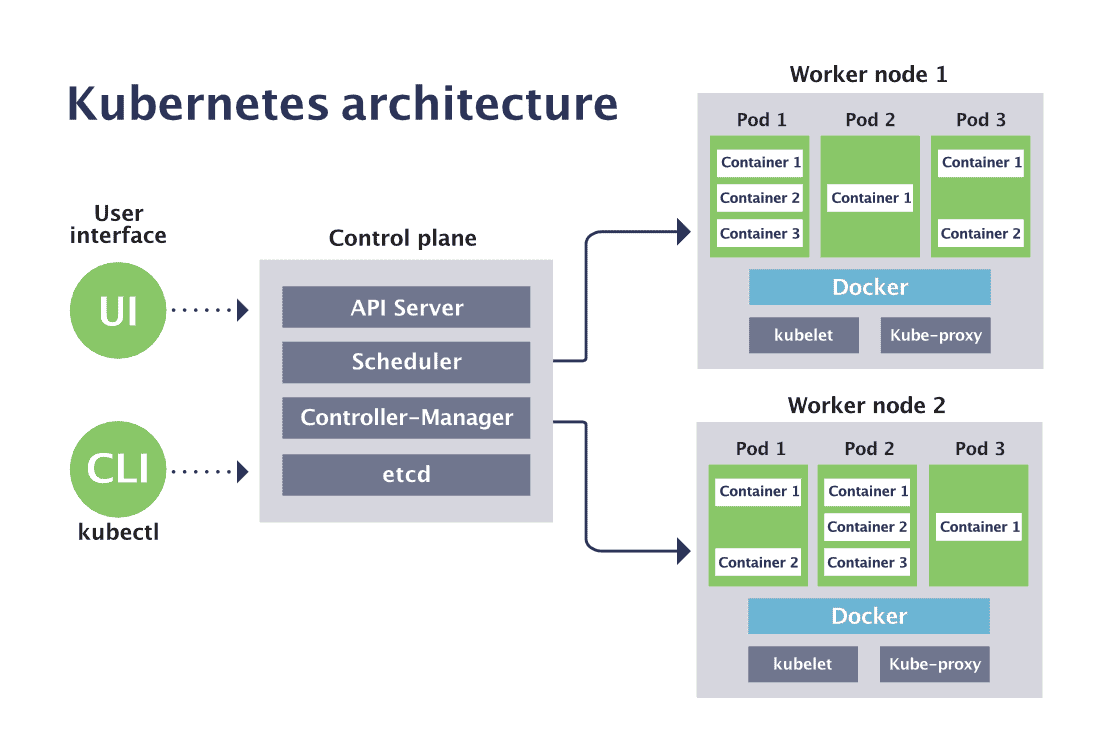
\includegraphics[width=0.9\linewidth]{uhu}
  \captionof{figure}{Deze afbeelding toont de verschillende onderdelen van een Kubernetes-cluster die moeten worden beschermd tegen ongeautoriseerde toegang, malware en andere zwakke punten.}
\end{center}

\begin{center}
    \captionsetup{type=figure}
    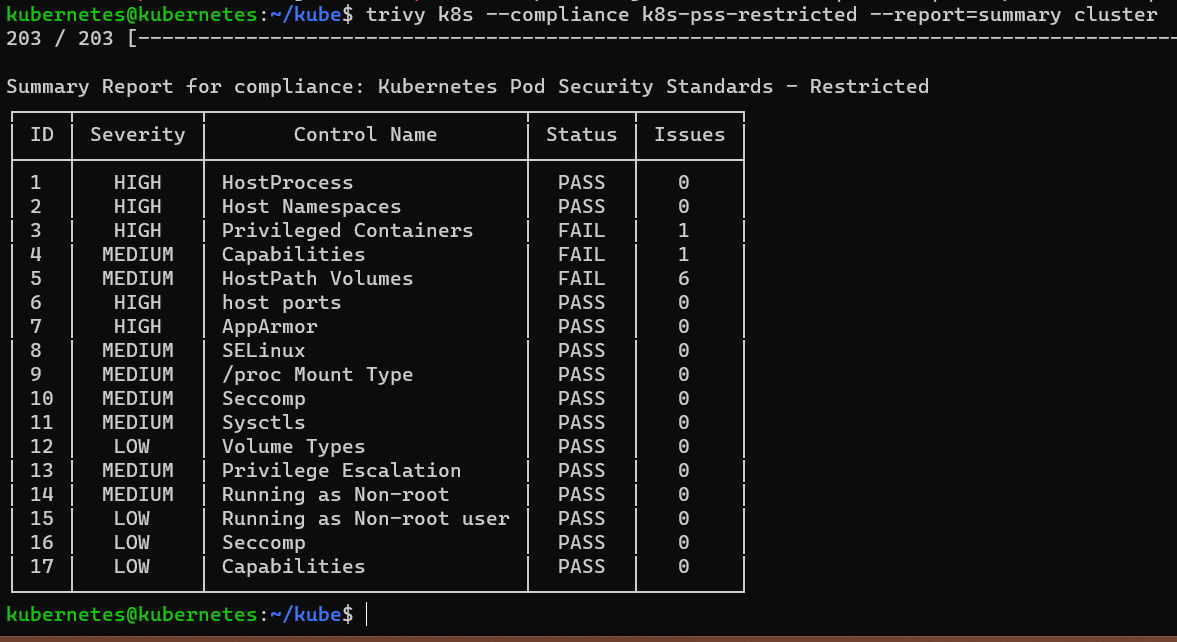
\includegraphics[width=1.0\linewidth]{complianceRestricted}
    \captionof{figure}{Het rapportresultaat van de Kubernetes-cluster, waarin wordt beoordeeld of een pod voldoet aan beperkte beveiligingsstandaarden, ook wel bekend als "Pod Security Standards, Restricted". Dit rapportresultaat is verkregen door het gebruik van de tool Trivy.}
\end{center}

\section{Conclusies}

Het beveiligen van een Kubernetes-omgeving vereist een combinatie van diverse tools, waaronder Kube-bench, Trivy en KubeLinter, om effectieve beveiliging te waarborgen. Het regelmatig updaten en patchen van het systeem is essentieel, samen met proactieve maatregelen zoals malware scanning en monitoring voor ongeautoriseerde toegang. OPA Gatekeeper kan helpen bij het implementeren van beleidsregels en het voorkomen van misconfiguraties. Deze tools bieden een verbeterde prestatie, gedetailleerde informatie over kwetsbaarheden en naleving van best practices, en samen omvatten ze een breed scala aan tactieken en technieken volgens de MITRE ATT\&CK matrix.

\section{Toekomstig onderzoek}

Toekomstig onderzoek kan zich richten op het verkennen van andere tools voor containerbeveiliging, netwerkmonitoringoplossingen en intrusion detection systemen. Het identificeren en evalueren van deze nieuwe technologieën kan waardevolle inzichten bieden om potentiële bedreigingen en aanvallen in een Kubernetes cluster te detecteren en te voorkomen, en zo de beveiliging van containerized applicaties verder te verbeteren.

\end{multicols}
\end{document}